         \chapter{Chemical bonding}\fancyfoot[LO,RE]{Chemistry: Matter and Materials}
    \setcounter{figure}{1}
    \setcounter{subfigure}{1}
    \label{m38704*cid1}
            \section{Introduction}
            \nopagebreak
            \label{m38704} $ \hspace{-5pt}\begin{array}{cccccccccccc}   
\includegraphics[width=0.75cm]{col11305.imgs/summary_fullmarks.png} &   \end{array} $ \hspace{2 pt}\raisebox{-5 pt}{} {(section shortcode: P10030 )} \par 
      \label{m38704*id138190}When you look at the matter, or physical substances, around you, you will realise that atoms seldom exist on their own. More often, the things around us are made up of different atoms that have been joined together. This is called \textbf{chemical bonding}. Chemical bonding is one of the most important processes in chemistry because it allows all sorts of different molecules and combinations of atoms to form, which then make up the objects in the complex world around us.\par 
    \label{m38704*cid4}
            \subsection*{What happens when atoms bond?}
            \nopagebreak
      \label{m38704*id138842}A \textbf{chemical bond} is formed when atoms are held together by attractive forces. This attraction occurs when electrons are \textsl{shared} between atoms, or when electrons are \textsl{exchanged} between the atoms that are involved in the bond. The sharing or exchange of electrons takes place so that the outer energy levels of the atoms involved are filled and the atoms are more stable. If an electron is \textbf{shared}, it means that it will spend its time moving in the electron orbitals around \textsl{both} atoms. If an electron is \textbf{exchanged} it means that it is transferred from one atom to another, in other words one atom \textsl{gains} an electron while the other \textsl{loses} an electron.\par 
\label{m38704*fhsst!!!underscore!!!id83}
\Definition{\label{id2427062}Chemical bond} {\label{m38704*meaningfhsst!!!underscore!!!id83} A chemical bond is the physical process that causes atoms and molecules to be attracted to each other, and held together in more stable chemical compounds.} 
      \label{m38704*id138909}The type of bond that is formed depends on the elements that are involved. In this chapter, we will be looking at three types of chemical bonding: \textbf{covalent}, \textbf{ionic} and \textbf{metallic bonding}.\par 
      \label{m38704*id138929}You need to remember that it is the \textsl{valence electrons} that are involved in bonding and that atoms will try to fill their outer energy levels so that they are more stable (or are more like the noble gases which are very stable).\par 
         \section{Lewis structures}
    \nopagebreak
            \label{m38701} $ \hspace{-5pt}\begin{array}{cccccccccccc}   
\includegraphics[width=0.75cm]{col11305.imgs/summary_fullmarks.png} &   \end{array} $ \hspace{2 pt}\raisebox{-5 pt}{} {(section shortcode: P10031 )} \par 
      \label{m38701*id140105}\textbf{Lewis notation} uses dots and crosses to represent the \textbf{valence electrons} on different atoms. The chemical symbol of the element is used to represent the nucleus and the core electrons of the atom.\par 
So, for example, a hydrogen atom would be represented like this: 
\begin{center}
\scalebox{0.8}{
\begin{pspicture}(1.5,1.5)(2.5,2.1)
%\psgrid[gridcolor=lightgray]
\rput(2,2){\Large \textbf{H}}
\rput(2.5,2){$\bullet$}
\end{pspicture}
}
\end{center}

A chlorine atom would look like this:
\begin{center}
\scalebox{0.8}{
\begin{pspicture}(-1,-0.6)(2,0.4)
%\psgrid[gridcolor=lightgray]
\rput(1,0){\Large \textbf{Cl}}
\uput{9pt}[d](1,0){$\times$ $\times$}
\rput{90}(1,0){\uput{9pt}[d](0,0){$\times$ $\times$}}
\rput{180}(1,0){\uput{9pt}[d](0,0){$\times$ $\times$}}
\rput{270}(1,0){\uput{9pt}[d](0,0){$\times$}}
\end{pspicture}
}
\end{center}

A molecule of hydrogen chloride would be shown like this:
\begin{center}
\scalebox{0.8}{
\begin{pspicture}(-1,-0.6)(2,0.6)
%\psgrid[gridcolor=lightgray]
\rput(1,0){\Large \textbf{Cl}}
\uput{9pt}[d](1,0){$\times$ $\times$}
\rput{90}(1,0){\uput{9pt}[d](0,0){$\times$ $\times$}}
\rput{180}(1,0){\uput{9pt}[d](0,0){$\times$ $\times$}}
\rput{270}(1,0){\uput{9pt}[d](0,0){$\times$ $\bullet$}}
\rput(0,0){\Large \textbf{H}}
\end{pspicture}
}
\end{center}

      \par 
      \label{m38701*id140178}The dot and cross in between the two atoms, represent the pair of electrons that are shared in the covalent bond.\par 
\label{m38701*secfhsst!!!underscore!!!id219}\vspace{.5cm}  
\begin{wex}{Lewis notation: Simple molecules\\}{Represent the molecule $H_{2}O$ using Lewis notation\\}
{\westep{For each atom, determine the number of valence electrons in the atom, and represent these using dots and crosses. }

The electron configuration of hydrogen is 1s$^{1}$ and the electron configuration for oxygen is 1s$^{2}$ 2s$^{2}$ 2p$^{4}$. Each hydrogen atom has one valence electron, which is unpaired, and the oxygen atom has six valence electrons with two unpaired.

\begin{figure}[H]
\begin{center}
\begin{pspicture}(-2,-0.5)(2,0.5)
%\psgrid[gridcolor=gray]
\rput(-1,0){\Large \textbf{H}}
\uput{10pt}[r](-1,0){$\bullet$}
\rput(1,0){\Large \textbf{O}}
\uput{9pt}[d](1,0){$\times$}
\rput{90}(1,0){\uput{9pt}[d](0,0){$\times$ $\times$}}
\rput{180}(1,0){\uput{9pt}[d](0,0){$\times$ $\times$}}
\rput{270}(1,0){\uput{9pt}[d](0,0){$\times$}}
\rput(-1.5,0){\Large 2}
\end{pspicture}
\end{center}
\end{figure}

\westep{Arrange the electrons so that the outermost energy level of each atom is full.}
The water molecule is represented below.

\begin{figure}[H]
\begin{center}
\begin{pspicture}(-0.2,-0.4)(2,0.4)
%\psgrid[gridcolor=gray]
\rput(0.1,0){\Large \textbf{H}}
\rput(1,0){\Large \textbf{O}}
\uput{9pt}[d](1,0){$\times$ $\bullet$}
\rput{90}(1,0){\uput{9pt}[d](0,0){$\times$ $\times$}}
\rput{180}(1,0){\uput{9pt}[d](0,0){$\times$ $\times$}}
\rput{270}(1,0){\uput{9pt}[d](0,0){$\times$ $\bullet$}}
\rput(1,-0.8){\Large \textbf{H}}
\end{pspicture}
\end{center}
\end{figure}
}
\end{wex}
    \noindent

\label{m38701*secfhsst!!!underscore!!!id245}\vspace{.5cm} 
      \noindent
\begin{wex}{Lewis notation: Molecules with multiple bonds\\}{Represent the molecule HCN using Lewis notation\\}
{\westep{For each atom, determine the number of valence electrons that the atom has from its electron configuration.}

The electron configuration of hydrogen is 1s$^{1}$, the electron configuration of nitrogen is 1s$^{2}$ 2s$^{2}$ 2p$^{3}$ and for carbon is 1s$^{2}$ 2s$^{2}$ 2p$^{2}$. This means that hydrogen has one valence electron which is unpaired, carbon has four valence electrons, all of which are unpaired, and nitrogen has five valence electrons, three of which are unpaired.

\begin{figure}[H]
\begin{center}
\begin{pspicture}(-2,-0.5)(4,0.5)
%\psgrid[gridcolor=gray]
\rput(-1,0){\Large \textbf{H}}
\uput{10pt}[r](-1,0){$\bullet$}
\rput(1,0){\Large \textbf{C}}
\uput{9pt}[d](1,0){$\times$}
\rput{90}(1,0){\uput{9pt}[d](0,0){$\times$}}
\rput{180}(1,0){\uput{9pt}[d](0,0){$\times$}}
\rput{270}(1,0){\uput{9pt}[d](0,0){$\times$}}
\rput(3,0){\Large \textbf{N}}
\uput{9pt}[d](3,0){$\bullet$}
\rput{90}(3,0){\uput{9pt}[d](0,0){$\bullet$}}
\rput{180}(3,0){\uput{9pt}[d](0,0){$\bullet$ $\bullet$}}
\rput{270}(3,0){\uput{9pt}[d](0,0){$\bullet$}}
\end{pspicture}
\end{center}
\end{figure}


\westep{Arrange the electrons in the HCN molecule so that the outermost energy level in each atom is full.}
The HCN molecule is represented below. Notice the three electron pairs between the nitrogen and carbon atom. Because these three covalent bonds are between the same two atoms, this is a \textit{triple} bond.

\begin{figure}[H]
\begin{center}
\begin{pspicture}(-2,-0.4)(4,0.4)
%\psgrid[gridcolor=gray]
\rput(0.1,0){\Large \textbf{H}}
\rput(1,0){\Large \textbf{C}}
\rput{270}(1,0){\uput{9pt}[d](0,0){$\times$ $\bullet$}}
\rput{90}(1,0){\uput{9pt}[d](0,0){$\times$ $\times$ $\times$}}
\rput(2,0){\Large \textbf{N}}
\rput{90}(2,0){\uput{9pt}[d](0,0){$\bullet$ $\bullet$}}
\rput{270}(2,0){\uput{9pt}[d](0,0){$\bullet$ $\bullet$ $\bullet$}}
\end{pspicture}
\end{center}
\end{figure}
}
\end{wex}
    \noindent
\label{m38701*secfhsst!!!underscore!!!id271}\vspace{.5cm} 
      \noindent
 \begin{wex}{Lewis notation: Atoms with variable valencies\\}{Represent the molecule H$_{2}$S using Lewis notation\\}

{\westep{Determine the number of valence electrons for each atom.}
Hydrogen has an electron configuration of 1s$^{1}$ and sulfur has an electron configuration of 1s$^{2}$ 2s$^{2}$ 2p$^{6}$ 3s$^{2}$ 3p$^{4}$. Each hydrogen atom has one valence electron which is unpaired, and sulfur has six valence electrons. Although sulfur has a variable valency, we know that the sulfur will be able to form 2 bonds with the hydrogen atoms. In this case, the valency of sulfur must be two.

\begin{figure}[H]
\begin{center}
\begin{pspicture}(-2,-0.4)(2,0.4)
%\psgrid[gridcolor=gray]
\rput(-1,0){\Large \textbf{H}}
\uput{10pt}[r](-1,0){$\bullet$}
\rput(-1.5,0){\Large 2}
\rput(1,0){\Large \textbf{S}}
\uput{9pt}[d](1,0){$\times$}
\rput{90}(1,0){\uput{9pt}[d](0,0){$\times$ $\times$}}
\rput{180}(1,0){\uput{9pt}[d](0,0){$\times$ $\times$}}
\rput{270}(1,0){\uput{9pt}[d](0,0){$\times$}}
\end{pspicture}
\end{center}
\end{figure}


\westep{Arrange the atoms in the molecule so that the outermost energy level in each atom is full.}
The H$_{2}$S molecule is represented below.\\

\begin{figure}[H]
\begin{center}
\begin{pspicture}(-0.2,-0.4)(2,0.4)
%\psgrid[gridcolor=gray]
\rput(0.1,0){\Large \textbf{H}}
\rput(1,0){\Large \textbf{S}}
\uput{9pt}[d](1,0){$\times$ $\bullet$}
\rput{90}(1,0){\uput{9pt}[d](0,0){$\times$ $\times$}}
\rput{180}(1,0){\uput{9pt}[d](0,0){$\times$ $\times$}}
\rput{270}(1,0){\uput{9pt}[d](0,0){$\times$ $\bullet$}}
\rput(1,-0.8){\Large \textbf{H}}
\end{pspicture}
\end{center}
\end{figure}
}
\end{wex}
    \noindent
\label{m38701*secfhsst!!!underscore!!!id327}
            \begin{exercises}{Lewis structures}
            \nopagebreak
      \label{m38701*id140889}\begin{enumerate}[noitemsep, label=\textbf{\arabic*}. ] 
            \label{m38701*uid23}\item Represent each of the following \textsl{atoms} using Lewis notation:
\label{m38701*id140910}\begin{enumerate}[noitemsep, label=\textbf{\alph*}. ] 
            \label{m38701*uid24}\item beryllium
\label{m38701*uid25}\item calcium
\label{m38701*uid26}\item lithium
\end{enumerate}
                \label{m38701*uid27}\item Represent each of the following \textsl{molecules} using Lewis notation:
\label{m38701*id140969}\begin{enumerate}[noitemsep, label=\textbf{\alph*}. ] 
            \label{m38701*uid28}\item bromine gas ($\mathrm{Br}{}_{2}$)
\label{m38701*uid29}\item carbon dioxide ($\mathrm{CO}{}_{2}$)
\end{enumerate}
                \label{m38701*uid30}\item Which of the two molecules listed above contains a double bond?\newline
\label{m38701*uid31}\item Two chemical reactions are described below.
\label{m38701*id141048}\begin{itemize}[noitemsep]
            \label{m38701*uid32}\item nitrogen and hydrogen react to form $\mathrm{NH}{}_{3}$\label{m38701*uid33}\item carbon and hydrogen bond to form a molecule of $\mathrm{CH}{}_{4}$\end{itemize}
For each reaction, give:
\label{m38701*id141106}\begin{enumerate}[noitemsep, label=\textbf{\alph*}. ] 
            \label{m38701*uid34}\item the valency of each of the atoms involved in the reaction
\label{m38701*uid35}\item the Lewis structure of the product that is formed
\label{m38701*uid36}\item the chemical formula of the product
\label{m38701*uid37}\item the name of the product
\end{enumerate}
                \label{m38701*uid38}\item A chemical compound has the following Lewis notation:
    \setcounter{subfigure}{0}
	\begin{figure}[H] % horizontal\label{m38701*id141174}
\begin{center}
\begin{pspicture}(1,-1)(2,0.4)
%\psgrid[gridcolor=gray]
\rput(0.1,0){\Large \textbf{X}}
\rput(1,0){\Large \textbf{Y}}
\uput{9pt}[d](1,0){$\times$ $\bullet$}
\rput{90}(1,0){\uput{9pt}[d](0,0){$\times$ $\times$}}
\rput{180}(1,0){\uput{9pt}[d](0,0){$\times$ $\times$}}
\rput{270}(1,0){\uput{9pt}[d](0,0){$\times$ $\bullet$}}
\rput(1,-0.8){\Large \textbf{H}}
\end{pspicture}
\end{center}
 \end{figure}       \label{m38701*id141181}\begin{enumerate}[noitemsep, label=\textbf{\alph*}. ] 
            \label{m38701*uid39}\item How many valence electrons does element $\mathrm{Y}$ have?
\label{m38701*uid40}\item What is the valency of element $\mathrm{Y}$?
\label{m38701*uid41}\item What is the valency of element $\mathrm{X}$?
\label{m38701*uid42}\item How many covalent bonds are in the molecule?
\label{m38701*uid43}\item Suggest a name for the elements $\mathrm{X}$ and $\mathrm{Y}$.
\end{enumerate}
                \end{enumerate}
  \label{m38701**end}
\par \raisebox{-5 pt}{
\includegraphics[width=0.5cm]{col11305.imgs/summary_www.png}} Find the answers with the shortcodes:
 \par \begin{tabular}[h]{cccccc}
 (1.) lOC  &  (2.) lOa  &  (3.) lOa  &  (4.) lOx  &  (5.) lOc  & \end{tabular}
\end{exercises}
    \label{m38704*cid5}
            \section{Covalent Bonding}
            \nopagebreak
            \label{m38704*uid6}
            \subsection*{The nature of the covalent bond}
            \nopagebreak
        \label{m38704*id138956}Covalent bonding occurs between the atoms of \textbf{non-metals}. The outermost orbitals of the atoms overlap so that unpaired electrons in each of the bonding atoms can be shared. By overlapping orbitals, the outer energy shells of all the bonding atoms are filled. The shared electrons move in the orbitals around \textsl{both} atoms. As they move, there is an attraction between these negatively charged electrons and the positively charged nuclei, and this force holds the atoms together in a covalent bond.\par 
\label{m38704*fhsst!!!underscore!!!id94}
\Definition{ \label{id2427171} Covalent bond} { \label{m38704*meaningfhsst!!!underscore!!!id94}
        Covalent bonding is a form of chemical bonding where pairs of electrons are shared between atoms.} 
        \label{m38704*id139505}You will have noticed in the above examples that the number of electrons that are involved in bonding varies between atoms. We say that the \textbf{valency} of the atoms is different.\par 
\label{m38704*fhsst!!!underscore!!!id165}
\Definition{ \label{id2427205}Valency} { \label{m38704*meaningfhsst!!!underscore!!!id165}
The number of electrons in the outer shell of an atom which are able to be used to form bonds with other atoms. } 
        \label{m38704*id139533}In the first example, the valency of both hydrogen and chlorine is one, therefore there is a single covalent bond between these two atoms. In the second example, nitrogen has a valency of three and hydrogen has a valency of one. This means that three hydrogen atoms will need to bond with a single nitrogen atom. There are three \textsl{single} covalent bonds in a molecule of ammonia. In the third example, the valency of oxygen is two. This means that each oxygen atom will form two bonds with another atom. Since there is only one other atom in a molecule of ${\mathrm{O}}_{2}$, a \textsl{double covalent} bond is formed between these two atoms.\par 
\label{m38704*notfhsst!!!underscore!!!id169}
\Tip {There is a relationship between the valency of an element and its position on the Periodic Table. For the elements in groups 1 to 4, the valency is the same as the group number. For elements in groups 5 to 7, the valency is calculated by subtracting the group number from 8. For example, the valency of fluorine (group 7) is $8-7=1$, while the valency of calcium (group 2) is 2. Some elements have more than one possible valency, so you always need to be careful when you are writing a chemical formula. Often, if there is more than one possibility in terms of valency, the valency will be written in a bracket after the element symbol e.g. carbon (IV) oxide, means that in this molecule carbon has a valency of 4.}
	\par
        \label{m38704*id138991}Below are a few examples. Remember that it is only the \textsl{valence electrons} that are involved in bonding, and so when diagrams are drawn to show what is happening during bonding, it is only these electrons that are shown. Circles and crosses are used to represent electrons in different atoms.\par 
\label{m38704*secfhsst!!!underscore!!!id98}\vspace{.5cm} 
\begin{wex}{Covalent bonding}{How do hydrogen and chlorine atoms bond covalently in a molecule of hydrogen chloride?}{\westep{Determine the electron configuration of each of the bonding atoms.}
A chlorine atom has 17 electrons, and an electron configuration of 1s$^{2}$ 2s$^{2}$ 2p$^{6}$ 3s$^{2}$ 3p$^{5}$. A hydrogen atom has only 1 electron, and an electron configuration of 1s$^{1}$.
\westep{Determine the number of valence electrons for each atom, and how many of the electrons are paired or unpaired.}
Chlorine has 7 valence electrons. One of these electrons is unpaired. Hydrogen has 1 valence electron and it is unpaired.
\westep{Look to see how the electrons can be shared between the atoms so that the outermost energy levels of both atoms are full.}
The hydrogen atom needs one more electron to complete its valence shell. The chlorine atom also needs one more electron to complete its shell. Therefore \textit{one pair of electrons} must be shared between the two atoms. In other words, one electron from the chlorine atom will spend some of its time orbiting the hydrogen atom so that hydrogen's valence shell is full. The hydrogen electron will spend some of its time orbiting the chlorine atom so that chlorine's valence shell is also full. A molecule of hydrogen chloride is formed. Notice the shared electron pair in the overlapping orbitals.
\begin{figure}[H]
\begin{center}
\scalebox{0.7}{
\begin{pspicture}(-7,-4.5)(7,1.5)
%\psgrid
\rput(-3.5,-1.8){\textbf{+}}
% Lower left
\uput[u](-5,-2){
\pscircle(0,0){1}
\qdisk(0.83,0.45){0.2}
\pscircle(3.5,0){1.5}
\uput{0}[u](0,-.2){\scalebox{2}{H}}

\rput(1.25,0){ 
\uput[d](0.83,-0.1){ \scalebox{2}{x}}
\uput{0.01}[l](2.25,1.5){ \scalebox{2}{x}}
\uput{0.01}[r](2.25,1.5){ \scalebox{2}{x}}
\uput[u](3.65,0){ \scalebox{2}{x}}
\uput[d](3.65,0){ \scalebox{2}{x}}
\uput{0.01}[l](2.25,-1.45){ \scalebox{2}{x}}
\uput{0.01}[r](2.25,-1.45){ \scalebox{2}{x}} 
\uput{0}[u](2.25,-.2){\scalebox{2}{Cl}}
}
}

% \psline{->}(0.5,2)(1.5,2)
\psline{->}(0.65,-2)(1.65,-2)

% Lower right
\uput[u](3,-2){
\pscircle(0,0){1}
\pscircle(2.25,0){1.5}
\qdisk(0.83,0.45){0.2}
\uput{0}[u](0,-.2){\scalebox{2}{H}}

\uput[d](0.83,-0.1){ \scalebox{2}{x}}
\uput{0.01}[l](2.25,1.5){ \scalebox{2}{x}}
\uput{0.01}[r](2.25,1.5){ \scalebox{2}{x}}
\uput[u](3.65,0){ \scalebox{2}{x}}
\uput[d](3.65,0){ \scalebox{2}{x}}
\uput{0.01}[l](2.25,-1.45){ \scalebox{2}{x}}
\uput{0.01}[r](2.25,-1.45){ \scalebox{2}{x}} 
\uput{0}[u](2.25,-.2){\scalebox{2}{Cl}}
}
\psline(-4,-1.5)(-3.5,-4)
\psline(-3,-2.5)(-3.5,-4)
\rput(-3.5,-4.4){\Large{unpaired electrons}}
\psline[arrows=<-](-1.5,0)(0,1)
\rput(2,1.5){\Large{paired electrons in valence energy level}}
\psline[arrows=<-](3.8,-2.6)(3.8,-4)
\rput(3.8,-4.5){\Large{overlap of electron orbitals and}}
\rput(3.8,-5){\Large{sharing of electron pair}}
\end{pspicture}
}
\end{center}
% \caption{Covalent bonding in a molecule of hydrogen chloride}
\label{fig:bonding:hydrogen chloride}
\end{figure}
}
\end{wex}
    \noindent
\par
\begin{wex}{Covalent bonding involving multiple bonds }{
 %problem
        \label{m38704*id139185}How do nitrogen and hydrogen atoms bond to form a molecule of ammonia ($\mathrm{NH}{}_{3}$)?\par 
        \vspace{5pt} 
}
{
%solution
\westep {Give the electron configuration}{ 
        \label{m38704*id139225}A nitrogen atom has 7 electrons, and an electron configuration of $1\mathrm{s}{}^{2}2\mathrm{s}{}^{2}2\mathrm{p}{}^{3}$. A hydrogen atom has only 1 electron, and an electron configuration of $1\mathrm{s}{}^{1}$.\par }
        \westep {Give the number of valence electrons}  {
        \label{m38704*id139283}Nitrogen has 5 valence electrons meaning that 3 electrons are unpaired. Hydrogen has 1 valence electron and it is unpaired.\par }
        \westep {Work out how the electrons are shared} {
        \label{m38704*id139292}Each hydrogen atom needs one more electron to complete its valence energy shell. The nitrogen atom needs three more electrons to complete its valence energy shell. Therefore \textsl{three pairs of electrons} must be shared between the four atoms involved. The nitrogen atom will share three of its electrons so that each of the hydrogen atoms now have a complete valence shell. Each of the hydrogen atoms will share its electron with the nitrogen atom to complete its valence shell.\par 
    \setcounter{subfigure}{0}
\begin{figure}[H]
\scalebox{0.7}{
\begin{pspicture}(-9,1)(9,7)
%\psgrid
\rput(-3.5,4.2){\textbf{+}}
% Upper left
\uput[u](-5,4){
\rput(-1.75,0.25){\scalebox{ 2}{ {\bf 3} }}
\pscircle(-0.25,0){1}
\qdisk(0.58,0.45){0.2}
\uput{0}[u](-0.25,-.2){\scalebox{2}{H}}

\rput(1.25,0){ 
\pscircle(2.25,0){1.5}
\uput[d](0.83,-0.1){ \scalebox{2}{x}} % left side

\uput{0.01}[l](2.25,1.5){ \scalebox{2}{x}} % top
\uput{0.01}[r](2.25,1.5){ \scalebox{2}{x}}

\uput[u](3.65,0){ \scalebox{2}{x}} % right side
\uput{0.01}[l](2.25,-1.45){ \scalebox{2}{x}} % bottom
\uput{0}[u](2.25,-.2){\scalebox{2}{N}} % N label
}
}

\psline{->}(0.5,4)(1.5,4)

% Upper right
\uput[u](3,4){
\rput(-0.25,0){ 
\pscircle(2.25,0){1.5}
\uput[d](0.83,-0.1){ \scalebox{2}{x}} % left side

\uput{0.01}[l](2.25,1.5){ \scalebox{2}{x}} % top
\uput{0.01}[r](2.25,1.5){ \scalebox{2}{x}}

\uput{0.3}[u](3.65,0){ \scalebox{2}{x}} % right side
\uput{0.1}[r](2.25,-1.4){ \scalebox{2}{x}} % bottom
\uput{0}[u](2.25,-.2){\scalebox{2}{N}} % N label
}
\rput(0,0){
\pscircle(-0.25,0){1}
\qdisk(0.58,0.45){0.2}
\uput{0}[u](-0.25,-.2){\scalebox{2}{H}}
} 
\rput(4.5,0){
\pscircle(-0.25,0){1}
\qdisk(-1.1,-0.45){0.2}
\uput{0}[u](-0.25,-.2){\scalebox{2}{H}}
} 
\rput(2.25,-2.25){
\pscircle(-0.25,0){1}
\qdisk(-0.75,0.9){0.2}
\uput{0}[u](-0.25,-.2){\scalebox{2}{H}}
} 
}
\end{pspicture}
}
\caption{Covalent bonding in a molecule of ammonia}
\label{fig:bonding:ammonia}
\end{figure}
} 
}
\end{wex}
    \noindent
        \label{m38704*id139334}The above examples all show \textbf{single covalent bonds}, where only one pair of electrons is shared between \textsl{the same two atoms}. If two pairs of electrons are shared between the same two atoms, this is called a \textbf{double bond}. A \textbf{triple bond} is formed if three pairs of electrons are shared.\par \pagebreak
\begin{wex}{Covalent bonding involving a double bond}{How do oxygen atoms bond covalently to form an oxygen molecule?\\}
{
\westep{Determine the electron configuration of the bonding atoms.}
Each oxygen atom has 8 electrons, and their electron configuration is 1s$^{2}$ 2s$^{2}$ 2p$^{4}$. 

\westep{Determine the number of valence electrons for each atom and how many of these electrons are paired and unpaired.}
Each oxygen atom has 6 valence electrons, meaning that each atom has 2 unpaired electrons.

\westep{Look to see how the electrons can be shared between atoms so that the outer energy shells of all the atoms are full.}

Each oxygen atom needs two more electrons to complete its valence energy shell. Therefore \textit{two pairs of electrons} must be shared between the two oxygen atoms so that both valence shells are full. Notice that the two electron pairs are being shared between \textit{the same two} atoms, and so we call this a \textbf{double bond}.

\begin{figure}[H]
\scalebox{0.7}{
\begin{pspicture}(-9,-4)(9,1)
 %\psgrid
\rput(-3.4,-1.8){\textbf{+}}
% Lower left
\uput[u](-5,-2){
\rput(-2.5,0){ 
\pscircle(2.25,0){1.5}
\uput[u](0.83,-0.1){ \scalebox{2}{x}} % left side
\uput[d](0.83,-0.1){ \scalebox{2}{x}} % left side

\uput{0.01}[l](2.25,1.5){ \scalebox{2}{x}} % top
\uput{0.01}[r](2.25,1.5){ \scalebox{2}{x}}

\uput[u](3.65,0){ \scalebox{2}{x}} % right side
\uput{0.01}[l](2.25,-1.45){ \scalebox{2}{x}} % bottom
\uput{0}[u](2.25,-.2){\scalebox{2}{O}} % O label
}
\rput(1.25,0){ 
\pscircle(2.25,0){1.5}
\uput[d](0.83,-0.1){ \qdisk(0,0){0.2} } % left side

\uput{0.3}[l](2.25,1.5){ \qdisk(0,0){0.2}} % top
\uput{0.3}[r](2.25,1.5){ \qdisk(0,0){0.2}}

\uput{0.3}[u](3.65,0){ \qdisk(0,0){0.2}} % right side
\uput{0.3}[d](3.65,0){ \qdisk(0,0){0.2}} % right side
\uput{0.3}[l](2.25,-1.45){ \qdisk(0,0){0.2}} % bottom
\uput{0}[u](2.25,-.2){\scalebox{2}{O}} % O label
}
}


\psline{->}(0.65,-2)(1.65,-2)


% Lower right
\uput[u](3,-2){
\rput(-1.5,0){ 
\pscircle(2.25,0){1.5}
\uput[u](0.83,-0.1){ \scalebox{2}{x}} % left side
\uput[d](0.83,-0.1){ \scalebox{2}{x}} % left side

\uput{0.01}[l](2.25,1.5){ \scalebox{2}{x}} % top
\uput{0.01}[r](2.25,1.5){ \scalebox{2}{x}}

\uput[u](3.4,0){ \scalebox{2}{x}} % right side
\uput[d](3.4,0){ \scalebox{2}{x}} % right side
\uput{0}[u](2.25,-.2){\scalebox{2}{O}} % O label
}
\rput(1.25,0){ 
\pscircle(2.25,0){1.5}
\uput{0.35}[u](1.06,-0.02){ \qdisk(0,0){0.2} } % left side
\uput{0.35}[d](1.06,-0.02){ \qdisk(0,0){0.2} } % left side

\uput{0.3}[l](2.25,1.5){ \qdisk(0,0){0.2}} % top
\uput{0.3}[r](2.25,1.5){ \qdisk(0,0){0.2}}

\uput{0.3}[u](3.65,0){ \qdisk(0,0){0.2}} % right side
\uput{0.3}[d](3.65,0){ \qdisk(0,0){0.2}} % right side
\uput{0}[u](2.25,-.2){\scalebox{2}{O}} % O label
}
}

\end{pspicture}
}
\label{fig:bonding:oxygen}
\end{figure}
}
\end{wex}
            \subsection*{Properties of covalent compounds}
            \nopagebreak
            \label{m38704*eip-541}
Covalent compounds have several properties that distinguish them from ionic compounds and metals. These properties are:
\label{m38704*di6325}\begin{enumerate}[noitemsep, label=\textbf{\arabic*}. ] 
            \item The melting and boiling points of covalent compounds is generally lower than that for ionic compounds.\item Covalent compounds are generally more flexible than ionic compounds. The molecules in covalent compounds are able to move around to some extent and can sometimes slide over each other (as is the case with graphite, this is why the lead in your pencil feels slightly slippery). In ionic compounds all the ions are tightly held in place.\item Covalent compounds generally are not very soluble in water.\item Covalent compounds generally do not conduct electricity when dissolved in water. This is because they do not dissociate as ionic compounds do.\end{enumerate}
\par 
    \noindent \vspace{-1cm}
\label{m38704*secfhsst!!!underscore!!!id172}
            \begin{exercises}{Covalent bonding and valency
        }
            \nopagebreak
        \label{m38704*id139588}\begin{enumerate}[noitemsep, label=\textbf{\arabic*}. ] 
            \label{m38704*uid10}\item Explain the difference between the \textsl{valence electrons} and the \textsl{valency} of an element.\newline
\label{m38704*uid11}\item Complete the table below by filling in the number of valence electrons and the valency for each of the elements shown:
    % \textbf{m38704*id139625}\par
          \begin{table}[H]
    % \begin{table}[H]
    % \\ 'id2897338' '1'
        \begin{center}
      \label{m38704*id139625}
    \noindent
      \begin{xtabular}{|l|l|l|l|}\hline
        \textbf{Element} & \textbf{No. of valence electrons} & \textbf{No. of electrons needed to fill outer shell} & \textbf{Valency} \\ \hline
        $\mathrm{F}$ & & & \\ \hline
        $\mathrm{Ar}$ & & & \\ \hline
        $\mathrm{C}$ & & & \\ \hline
        $\mathrm{N}$ & & & \\ \hline
        $\mathrm{O}$ & & & \\ \hline
    \end{tabular}
      \end{center}
\end{table}
    \par
          \label{m38704*uid12}\item Draw simple diagrams to show how electrons are arranged in the following covalent molecules:
\label{m38704*id140030}\begin{enumerate}[noitemsep, label=\textbf{\alph*}. ] 
            \label{m38704*uid13}\item Water ($\mathrm{H}{}_{2}\mathrm{O}$)
\label{m38704*uid14}\item Chlorine ($\mathrm{Cl}{}_{2}$)
\end{enumerate}
                \end{enumerate}
      \label{m38704*eip-790}
\par \raisebox{-5 pt}{
\includegraphics[width=0.5cm]{col11305.imgs/summary_www.png}} Find the answers with the shortcodes:
 \par \begin{tabular}[h]{cccccc}
 (1.) lOY  &  (2.) lOr  &  (3.) lO1  & \end{tabular}
\end{exercises}

         \section{Ionic bonding}
    \nopagebreak
            \label{m38684} $ \hspace{-5pt}\begin{array}{cccccccccccc}   \end{array} $ \hspace{2 pt}\raisebox{-5 pt}{
\includegraphics[width=0.5cm]{col11305.imgs/summary_www.png}} {(section shortcode: P10032 )} \par 
      \label{m38684*uid54}
            \subsection*{The nature of the ionic bond}
            \nopagebreak
        \label{m38684*id142190}You will remember that when atoms bond, electrons are either \textsl{shared} or they are \textsl{transferred} between the atoms that are bonding. In covalent bonding, electrons are shared between the atoms. There is another type of bonding, where electrons are \textsl{transferred} from one atom to another. This is called \textbf{ionic bonding}.\par 
        \label{m38684*id142218}Ionic bonding takes place when the difference in electronegativity between the two atoms is more than 1,7. This usually happens when a metal atom bonds with a non-metal atom. When the difference in electronegativity is large, one atom will attract the shared electron pair much more strongly than the other, causing electrons to be transferred from one atom to the other.\par 
\label{m38684*fhsst!!!underscore!!!id456}
\Definition{   \label{id2430088} Ionic bond } { \label{m38684*meaningfhsst!!!underscore!!!id456}
        An ionic bond is a type of chemical bond based on the electrostatic forces between two oppositely-charged ions. When ionic bonds form, a metal donates one or more electrons, due to having a low electronegativity, to form a positive ion or cation. The non-metal atom has a high electronegativity, and therefore readily gains electrons to form a negative ion or anion. The two ions are then attracted to each other by electrostatic forces.
         } 
        \label{m38684*id142248}
          \textbf{Example 1:}
        \par 
        \label{m38684*id142255}In the case of $\mathrm{NaCl}$, the difference in electronegativity is 2,1. Sodium has only one valence electron, while chlorine has seven. Because the electronegativity of chlorine is higher than the electronegativity of sodium, chlorine will attract the valence electron of the sodium atom very strongly. This electron from sodium is transferred to chlorine. Sodium loses an electron and forms an ${\mathrm{Na}}^{+}$ ion. Chlorine gains an electron and forms an ${\mathrm{Cl}}^{-}$ ion. The attractive force between the positive and negative ion holds the molecule together.\par 
        \label{m38684*id142300}The balanced equation for the reaction is:\par 
        \label{m38684*id142305}\nopagebreak\noindent{}
    \begin{equation}
    \mathrm{Na}+\mathrm{Cl}\to \mathrm{NaCl}\tag{5.1}
      \end{equation}
        \label{m38684*id142337}This can be represented using Lewis notation:\par 
    \setcounter{subfigure}{0}
\begin{figure}[!h]
\begin{center}
\begin{pspicture}(-3,-1.4)(6,1)
		%\psgrid
		\psline[linearc=0.25]{->}(-1.5,-0.2)(-1.2,-0.6)(-0.8,-0.2)
		\rput(-1.2,-0.8){electron transer from}
		\rput(-1.2,-1.1){sodium to chlorine}
		\rput(-1.1,0){\textbf{+}}
		\rput(-2.1,0){ \scalebox{2}{Na}}
		\uput{15pt}[r](-2.1,0){$\bullet$}
		\rput(-0.3,0){
			\uput{0.05}[l](0,0.5){$\times$}		% Top
			\uput{0.05}[r](0,0.5){$\times$}
			\uput{0.05}[u](0.5,0){$\times$}		% Right
			\uput{0.05}[d](0.5,0){$\times$}
			\uput{0.05}[l](0,-0.5){$\times$}		% Bottom
			\uput{0.05}[r](0,-0.5){$\times$}	
			\uput{0.05}[u](-0.5,0){$\times$}		% Left			
			\rput(-0.2,0){ \scalebox{2}{Cl}}

		}

		\psline[arrowsize=0.2]{->}(0.75,0)(1.75,0)
		
		\rput(4.05,0){ \scalebox{2}{[Na]$ ^+ $[\hspace{0.02cm}  Cl \hspace{0.02cm}]$^-$} }
		\rput(4.7,0){
			\uput{0.05}[l](0,0.5){$\times$}		% Top
			\uput{0.05}[r](0,0.5){$\times$}
			\uput{0.05}[u](0.5,0){$\times$}		% Right
			\uput{0.05}[d](0.5,0){$\times$}
			\uput{0.05}[l](0,-0.5){$\times$}		% Bottom
			\uput{0.05}[r](0,-0.5){$\times$}	
			\uput{0.05}[u](-0.5,0){$\times$}		% Left			
			\uput{0.05}[d](-0.5,0){$\bullet$}
		}
		
	\end{pspicture}
	
\caption{Ionic bonding in sodium chloride}
\end{center}
\end{figure}       
        \label{m38684*id142353}
          \textbf{Example 2:}
        \par 
        \label{m38684*id142360}Another example of ionic bonding takes place between magnesium ($\mathrm{Mg}$) and oxygen ($\mathrm{O}$) to form magnesium oxide ($\mathrm{MgO}$). Magnesium has two valence electrons and an electronegativity of 1,2, while oxygen has six valence electrons and an electronegativity of 3,5. Since oxygen has a higher electronegativity, it attracts the two valence electrons from the magnesium atom and these electrons are transferred from the magnesium atom to the oxygen atom. Magnesium loses two electrons to form ${\mathrm{Mg}}^{2+}$, and oxygen gains two electrons to form ${\mathrm{O}}^{2-}$. The attractive force between the oppositely charged ions is what holds the molecule together.\par 
        \label{m38684*id138529}The balanced equation for the reaction is:\par 
        \label{m38684*id138535}\nopagebreak\noindent{}
    \begin{equation}
    2\mathrm{Mg}+{\mathrm{O}}_{2}\to 2\mathrm{MgO}\tag{5.2}
      \end{equation}
        \label{m38684*id142521}Because oxygen is a diatomic molecule, two magnesium atoms will be needed to combine with one oxygen molecule (which has two oxygen atoms) to produce two molecules of magnesium oxide ($\mathrm{MgO}$).\par 
    \setcounter{subfigure}{0}
\begin{figure}[!h]
\begin{center}
\begin{pspicture}(-3,-1.2)(6,1)
		%\psgrid
		\psline[linearc=0.25]{->}(-1.8,0.6)(-1.2,0.8)(-0.7,0)
		\psline[linearc=0.25]{->}(-1.2,-0.2)(-0.6,-0.6)(-0.2,-0.4)
		\rput(-1,-1){two electrons transferred}
		\rput(-1,-1.3){from Mg to O}
		\rput(-2,0){ \scalebox{2} {Mg}}
		\uput{17pt}[r](-2,0){$\bullet$}
		\uput{12pt}[u](-2,0){$\bullet$}

		\rput(0,0){ \scalebox{2} {O}}

		\rput(0,0){
			\uput{0.05}[l](0,0.5){$\times$}		% Top
			\uput{0.05}[r](0,0.5){$\times$}
			\uput{0.05}[u](0.5,0){$\times$}		% Right
			\uput{0.05}[d](0.5,0){$\times$}
			\uput{0.05}[r](0,-0.5){$\times$}	
			\uput{0.05}[u](-0.5,0){$\times$}		% Left			
			
		}
		\psline[arrowsize=0.2]{->}(0.75,0)(1.75,0)
		
		\rput(4.35,0){ \scalebox{2}{[Mg]$ ^{2+} $[\hspace{0.1cm}  O \hspace{0.1cm}]$^{2-}$} }
		\rput(5,0){
			\uput{0.05}[l](0,0.5){$\times$}		% Top
			\uput{0.05}[r](0,0.5){$\times$}
			\uput{0.05}[u](0.5,0){$\times$}		% Right
			\uput{0.05}[d](0.5,0){$\times$}
			\uput{0.1}[l](0,-0.5){$\bullet$}		% Bottom
			\uput{0.05}[r](0,-0.5){$\times$}	
			\uput{0.05}[u](-0.5,0){$\times$}		% Left			
			\uput{0.1}[d](-0.5,0){$\bullet$}
		}
		
	\end{pspicture}
	
\end{center}		
\caption{Ionic bonding in magnesium oxide}
\end{figure}       
\label{m38684*notfhsst!!!underscore!!!id521}
\Tip{Notice that the number of electrons that is either lost or gained by an atom during ionic bonding, is the same as the \textbf{valency} of that element}
	\par
\label{m38684*secfhsst!!!underscore!!!id522}
            \begin{exercises}{Ionic compounds
        }
            \nopagebreak
        \label{m38684*id142562}\begin{enumerate}[noitemsep, label=\textbf{\arabic*}. ] 
            \label{m38684*uid57}\item Explain the difference between a \textsl{covalent} and an \textsl{ionic} bond.\newline
\label{m38684*uid58}\item Magnesium and chlorine react to form magnesium chloride.
\label{m38684*id142602}\begin{enumerate}[noitemsep, label=\textbf{\alph*}. ] 
            \label{m38684*uid59}\item What is the difference in electronegativity between these two elements?
\label{m38684*uid60}\item Give the chemical formula for:
\label{m38684*id142630}\begin{enumerate}[noitemsep, label=\textbf{\roman*}. ] 
            \label{m38684*uid61}\item a magnesium ion
\label{m38684*uid62}\item a chloride ion
\label{m38684*uid63}\item the ionic compound that is produced during this reaction
\end{enumerate}
        \label{m38684*uid64}\item Write a balanced chemical equation for the reaction that takes place.
\end{enumerate}
        \label{m38684*uid65}\item Draw Lewis diagrams to represent the following ionic compounds:
\label{m38684*id142697}\begin{enumerate}[noitemsep, label=\textbf{\alph*}. ] 
            \label{m38684*uid66}\item sodium iodide ($\mathrm{NaI}$)
\label{m38684*uid67}\item calcium bromide ($\mathrm{CaBr}{}_{2}$)
\label{m38684*uid68}\item potassium chloride ($\mathrm{KCl}$)
\end{enumerate}
        \end{enumerate}
      \label{m38684*uid69}
\par \raisebox{-5 pt}{
\includegraphics[width=0.5cm]{col11305.imgs/summary_www.png}} Find the answers with the shortcodes:
 \par \begin{tabular}[h]{cccccc}
 (1.) lOq  &  (2.) lOl  &  (3.) lOi  & \end{tabular}
\end{exercises}
            \subsection{The crystal lattice structure of ionic compounds}
            \nopagebreak
        \label{m38684*id142771}Ionic substances are actually a combination of lots of ions bonded
together into a giant molecule. The arrangement of ions in a regular,
geometric structure is called a \textbf{crystal lattice}. So in
fact $\mathrm{NaCl}$ does not contain one $\mathrm{Na}$ and one $\mathrm{Cl}$ ion, but rather a lot of
these two ions arranged in a crystal lattice where the ratio of $\mathrm{Na}$ to
$\mathrm{Cl}$ ions is 1:1. The structure of a crystal lattice is shown in Figure~5.18.\par 
\begin{minipage}{.5\textwidth}
    \setcounter{subfigure}{0}
% \begin{figure}[h]
\begin{center}
\scalebox{.8}{
\begin{pspicture}(-3,-3)(3,3)
%\psgrid
\psline(2.4,2.4)(4.4,2.4)
\rput(6.5,2.4){atom of element 1 (e.g. Na)}
\psline(2.4,0.4)(4.4,0.4)
\rput(6.5,0.4){atom of element 2 (e.g. Cl)}
\psline(2.2,-1.8)(4.4,-1.8)
\rput(6.8,-1.8){ionic bonds hold atoms together}
\rput(6.8,-2.2){in the lattice structure}

  \psset{Alpha=75,Beta=20}
  \psset{xMin=-3,xMax=3,yMin=-3,yMax=3,zMin=-3,zMax=3}
%   \pstThreeDCoor
   \pstThreeDLine(-2,-2,-2)(-2,-2,2) \pstThreeDLine(-2,-2,2)(-2,2,2)
   \pstThreeDLine(-2,2,2)(-2,2,-2) \pstThreeDLine(-2,2,-2)(-2,-2,-2)
   \pstThreeDLine(-2,-2,0)(-2,2,0) \pstThreeDLine(-2,0,-2)(-2,0,2)

   \pstThreeDLine(0,-2,-2)(0,-2,2) \pstThreeDLine(0,-2,2)(0,2,2)
   \pstThreeDLine(0,2,2)(0,2,-2) \pstThreeDLine(0,2,-2)(0,-2,-2)
   \pstThreeDLine(0,-2,0)(0,2,0) \pstThreeDLine(0,0,-2)(0,0,2)

  \pstThreeDLine(2,-2,-2)(2,-2,2) \pstThreeDLine(2,-2,2)(2,2,2)
  \pstThreeDLine(2,2,2)(2,2,-2) \pstThreeDLine(2,2,-2)(2,-2,-2)
  \pstThreeDLine(2,-2,0)(2,2,0) \pstThreeDLine(2,0,-2)(2,0,2)

  \pstThreeDLine(-2,2,2)(2,2,2) \pstThreeDLine(-2,0,2)(2,0,2)
  \pstThreeDLine(-2,-2,2)(2,-2,2)
  \pstThreeDLine(-2,2,0)(2,2,0) \pstThreeDLine(-2,0,0)(2,0,0)
  \pstThreeDLine(-2,-2,0)(2,-2,0)
  \pstThreeDLine(-2,2,-2)(2,2,-2) \pstThreeDLine(-2,0,-2)(2,0,-2)
  \pstThreeDLine(-2,-2,-2)(2,-2,-2)

  \SpecialCoor
  \psset{dotstyle=*,dotscale=3.2}
  \pstThreeDDot(-2,-2,-2)\pstThreeDDot(-2,2,-2)\pstThreeDDot( 0,0,-2)
  \pstThreeDDot( 2,-2,-2)\pstThreeDDot( 2,2,-2)
  \pstThreeDDot(-2,0, 0)\pstThreeDDot( 0,-2, 0)\pstThreeDDot( 0,2, 0)
  \pstThreeDDot( 2,0, 0)
  \pstThreeDDot(-2,-2, 2)\pstThreeDDot(-2,2, 2)\pstThreeDDot( 0,0, 2)
  \pstThreeDDot( 2,-2, 2)\pstThreeDDot( 2,2, 2)

  \psset{dotstyle=o,dotscale=3}
  \pstThreeDDot(-2,0,-2)\pstThreeDDot( 0,-2,-2)\pstThreeDDot( 0,2,-2)
  \pstThreeDDot( 2,0,-2)
  \pstThreeDDot(-2,-2, 0)\pstThreeDDot(-2,2, 0)\pstThreeDDot( 0,0, 0)
  \pstThreeDDot( 2,-2, 0)\pstThreeDDot( 2,2, 0)
  \pstThreeDDot(-2,0, 2)\pstThreeDDot( 0,-2, 2)\pstThreeDDot( 0,2, 2)
  \pstThreeDDot( 2,0, 2)

%  \psgrid
\end{pspicture}
}
\end{center}
% \caption{The crystal lattice arrangement in an ionic compound (e.g. NaCl)}
% \label{fig:atomcomb:crystal lattice}
% \end{figure}       
\end{minipage}
\begin{minipage}{.5\textwidth}
 \begin{center}
  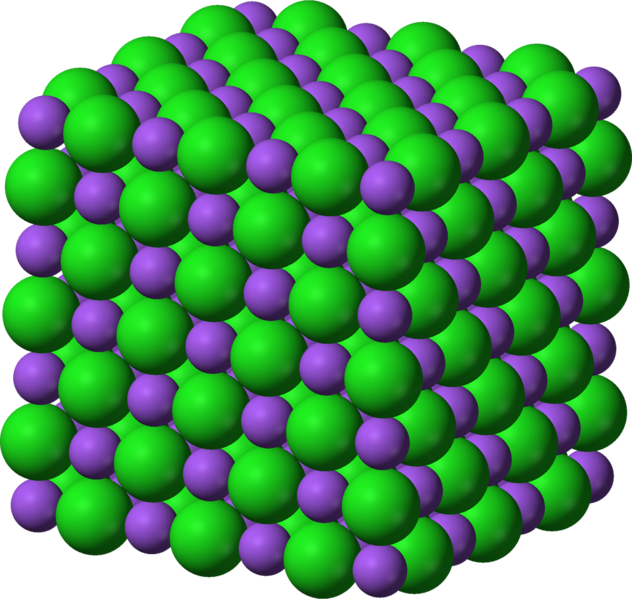
\includegraphics[width=0.5\textwidth]{photos/sodiumchloride_wikipedia.png}
 \end{center}

\end{minipage}

      \label{m38684*uid71}
            \subsection{Properties of Ionic Compounds}
            \nopagebreak
        \label{m38684*id142811}Ionic compounds have a number of properties:\par 
        \label{m38684*id142815}\begin{itemize}[noitemsep]
            \label{m38684*uid72}\item Ions are arranged in a lattice structure
\label{m38684*uid73}\item Ionic solids are crystalline at room temperature
\label{m38684*uid74}\item The ionic bond is a strong electrical attraction. This means that ionic compounds are often hard and have high melting and boiling points
\label{m38684*uid75}\item Ionic compounds are brittle, and bonds are broken along planes when the compound is stressed
\label{m38684*uid76}\item Solid crystals don't conduct electricity, but ionic solutions do
\end{itemize}
  \label{m38684**end}
         \section{Metallic Bonding}
    \nopagebreak
            \label{m38694} $ \hspace{-5pt}\begin{array}{cccccccccccc}   
\includegraphics[width=0.75cm]{col11305.imgs/summary_video.png} &   \end{array} $ \hspace{2 pt}\raisebox{-5 pt}{} {(section shortcode: P10033 )} \par 
      \label{m38694*uid77}
            \subsection{The nature of the metallic bond}
            \nopagebreak
        \label{m38694*id142901}The structure of a metallic bond is quite different from covalent and ionic bonds. In a metal bond, the valence electrons are \textsl{delocalised}, meaning that an atom's electrons do not stay around that one nucleus. In a metallic bond, the positive atomic nuclei (sometimes called the 'atomic kernels') are surrounded by a sea of delocalised electrons which are attracted to the nuclei (Figure~5.19).\par 
\label{m38694*fhsst!!!underscore!!!id582}
\Definition{ \label{id2431026} Metallic bond} { \label{m38694*meaningfhsst!!!underscore!!!id582}
Metallic bonding is the electrostatic attraction between the positively charged atomic nuclei of metal atoms and the delocalised electrons in the metal.}
\begin{minipage}{.5\textwidth}
    \setcounter{subfigure}{0}
% \begin{figure}[h]
\begin{center}
\scalebox{0.8}{
\begin{pspicture}(-3,-3)(3,3)
\psframe(0,0)(5,5)
%row 1
\multirput(1,1)(1,0){4}{
\pscircle(0,0){.2}
\uput[r]{0}(-0.3,0){$+$}}
\multirput(0.5,0.5)(1,0){5}{\qdisk(0,0){2pt}}
%row 2
\pscircle(1,2){.2}
\uput[r]{0}(0.7,2){$+$}
\pscircle(2,2){.2}
\uput[r]{0}(1.7,2){$+$}
\pscircle(3,2){.2}
\uput[r]{0}(2.7,2){$+$}
\pscircle(4,2){.2}
\uput[r]{0}(3.7,2){$+$}
\multirput(0.5,1.5)(1,0){5}{\qdisk(0,0){2pt}}
%row 3
\pscircle(1,3){.2}
\uput[r]{0}(0.7,3){$+$}
\pscircle(2,3){.2}
\uput[r]{0}(1.7,3){$+$}
\pscircle(3,3){.2}
\uput[r]{0}(2.7,3){$+$}
\pscircle(4,3){.2}
\uput[r]{0}(3.7,3){$+$}
\multirput(0.5,2.5)(1,0){5}{\qdisk(0,0){2pt}}
%row 4
\pscircle(1,4){.2}
\uput[r]{0}(0.7,4){$+$}
\pscircle(2,4){.2}
\uput[r]{0}(1.7,4){$+$}
\pscircle(3,4){.2}
\uput[r]{0}(2.7,4){$+$}
\pscircle(4,4){.2}
\uput[r]{0}(3.7,4){$+$}
\multirput(0.5,3.5)(1,0){5}{\qdisk(0,0){2pt}}
\multirput(0.5,4.5)(1,0){5}{\qdisk(0,0){2pt}}
\end{pspicture}
}
\end{center}
% \caption{Positive atomic nuclei (+) surrounded by delocalised electrons ($\bullet$)}
% \label{fig:an:metallic bond}
% \end{figure}      
\end{minipage}
\begin{minipage}{.5\textwidth}
 \begin{center}
  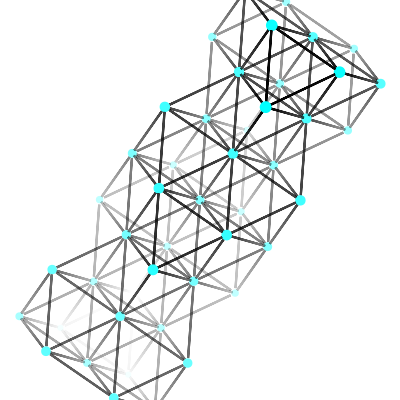
\includegraphics[width=0.6\textwidth]{photos/copper_structure.png}
 \end{center}

\end{minipage}

        \label{m38694*id754}
            \begin{activity}{Building models}
            \nopagebreak
        \label{m38694*id87434}Using coloured balls and sticks (or any other suitable materials) build models of each type of bonding. Think about how to represent each kind of bonding. For example, covalent bonding could be represented by simply connecting the balls with sticks to represent the molecules, while for ionic bonding you may wish to construct part of the crystal lattice. Do some research on types of crystal lattices (although the section on ionic bonding only showed the crystal lattice for sodium chloride, many other types of lattices exist) and try to build some of these. Share your findings with your class and compare notes to see what types of crystal lattices they found. How would you show metallic bonding?\par 
        \label{m38694*id8754}You should spend some time doing this activity as it will really help you to understand how atoms combine to form molecules and what the differences are between the types of bonding. \par 
\end{activity}
\label{m38694*eip-515}
    \setcounter{subfigure}{0}
	\begin{figure}[H] % horizontal\label{m38694*bonds-1}
    \textnormal{Khan academy video on bonding - 1}\vspace{.1in} \nopagebreak
  \label{m38694*yt-media1}\label{m38694*yt-video1}
            \raisebox{-5 pt}{ 
\includegraphics[width=0.5cm]{col11305.imgs/summary_www.png}} { (Video:  P10034 )}
      \vspace{2pt}
    \vspace{.1in}
 \end{figure}       \par \label{m38694*secfhsst!!!underscore!!!id617}
            \begin{exercises}{  Chemical bonding
        }
            \nopagebreak
        \label{m38694*id143111}\begin{enumerate}[noitemsep, label=\textbf{\arabic*}. ] 
            \label{m38694*uid86}\item Give two examples of everyday objects that contain..
\label{m38694*id143127}\begin{enumerate}[noitemsep, label=\textbf{\alph*}. ] 
            \label{m38694*uid87}\item covalent bonds
\label{m38694*uid88}\item ionic bonds
\label{m38694*uid89}\item metallic bonds
\end{enumerate}
                \label{m38694*uid90}\item Complete the table which compares the different types of bonding:
    % \textbf{m38694*id143180}\par
          \begin{table}[H]
    % \begin{table}[H]
    % \\ 'id2900564' '1'
        \begin{center}
      \label{m38694*id143180}
    \noindent
    \tabletail{%
        \hline
        \multicolumn{4}{|p{\mytableboxwidth}|}{\raggedleft \small \sl continued on next page}\\
        \hline
      }
      \tablelasttail{}
      \begin{xtabular}[t]{|l|l|l|l|}\hline
         &
        \textbf{Covalent} &
        \textbf{Ionic} &
        \textbf{Metallic}% make-rowspan-placeholders
     \tabularnewline\cline{1-1}\cline{2-2}\cline{3-3}\cline{4-4}
      %--------------------------------------------------------------------
        Types of atoms involved &
         &
         &
        % make-rowspan-placeholders
     \tabularnewline\cline{1-1}\cline{2-2}\cline{3-3}\cline{4-4}
      %--------------------------------------------------------------------
        Nature of bond between atoms &
         &
         &
        % make-rowspan-placeholders
     \tabularnewline\cline{1-1}\cline{2-2}\cline{3-3}\cline{4-4}
      %--------------------------------------------------------------------
        Melting Point (high/low) &
         &
         &
        % make-rowspan-placeholders
     \tabularnewline\cline{1-1}\cline{2-2}\cline{3-3}\cline{4-4}
      %--------------------------------------------------------------------
        Conducts electricity? (yes/no) &
         &
         &
        % make-rowspan-placeholders
     \tabularnewline\cline{1-1}\cline{2-2}\cline{3-3}\cline{4-4}
      %--------------------------------------------------------------------
        Other properties &
         &
         &
        % make-rowspan-placeholders
     \tabularnewline\cline{1-1}\cline{2-2}\cline{3-3}\cline{4-4}
      %--------------------------------------------------------------------
    \end{xtabular}
      \end{center}
\end{table}
    \par
          \label{m38694*uid91}\item Complete the table below by identifying the type of bond (covalent, ionic or metallic) in each of the compounds:
    % \textbf{m38694*id143418}\par
          \begin{table}[H]
    % \begin{table}[H]
    % \\ 'id2900649' '1'
        \begin{center}
      \label{m38694*id143418}
    \noindent
    \tabletail{%
        \hline
        \multicolumn{2}{|p{\mytableboxwidth}|}{\raggedleft \small \sl continued on next page}\\
        \hline
      }
      \tablelasttail{}
      \begin{xtabular}[t]{|l|l|}\hline
        \textbf{Molecular formula} &
        \textbf{Type of bond}% make-rowspan-placeholders
     \tabularnewline\cline{1-1}\cline{2-2}
      %--------------------------------------------------------------------
        $\mathrm{H}{}_{2}\mathrm{SO}{}_{4}$ &
        % make-rowspan-placeholders
     \tabularnewline\cline{1-1}\cline{2-2}
      %--------------------------------------------------------------------
        $\mathrm{FeS}$ &
        % make-rowspan-placeholders
     \tabularnewline\cline{1-1}\cline{2-2}
      %--------------------------------------------------------------------
        $\mathrm{NaI}$ &
        % make-rowspan-placeholders
     \tabularnewline\cline{1-1}\cline{2-2}
      %--------------------------------------------------------------------
        $\mathrm{MgCl}{}_{2}$ &
        % make-rowspan-placeholders
     \tabularnewline\cline{1-1}\cline{2-2}
      %--------------------------------------------------------------------
        $\mathrm{Zn}$ &
        % make-rowspan-placeholders
     \tabularnewline\cline{1-1}\cline{2-2}
      %--------------------------------------------------------------------
    \end{xtabular}
      \end{center}
\end{table}
    \par
          \label{m38694*uid92}\item Which of these substances will conduct electricity most effectively? Give a reason for your answer.\newline
\label{m38694*uid93}\item Use your knowledge of the different types of bonding to explain the following statements:
\label{m38694*id143618}\begin{enumerate}[noitemsep, label=\textbf{\alph*}. ] 
            \label{m38694*uid94}\item Swimming during an electric storm (i.e. where there is lightning) can be very dangerous.
\label{m38694*uid95}\item Most jewellery items are made from metals.
\label{m38694*uid96}\item Plastics are good insulators.
\end{enumerate}
                \end{enumerate}
  \label{m38694**end}
\par \raisebox{-5 pt}{
\includegraphics[width=0.5cm]{col11305.imgs/summary_www.png}} Find the answers with the shortcodes:
 \par \begin{tabular}[h]{cccccc}
 (1.) l3h  &  (2.) l3u  &  (3.) l3J  &  (4.) l3J  &  (5.) l3S  & \end{tabular}
\end{exercises}
         \section{Writing formulae}
    \nopagebreak
            \label{m38689} $ \hspace{-5pt}\begin{array}{cccccccccccc}   
\includegraphics[width=0.75cm]{col11305.imgs/summary_fullmarks.png} &   
\includegraphics[width=0.75cm]{col11305.imgs/summary_video.png} &   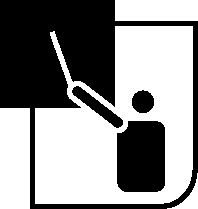
\includegraphics[width=0.75cm]{col11305.imgs/summary_presentation.png} &   \end{array} $ \hspace{2 pt}\raisebox{-5 pt}{} {(section shortcode: P10035 )} \par 
      \label{m38689*uid97}
            \subsection{The formulae of covalent compounds}
            \nopagebreak
        \label{m38689*id143689}To work out the formulae of covalent compounds, we need to use the valency of the atoms in the compound. This is because the valency tells us how many bonds each atom can form. This in turn can help to work out how many atoms of each element are in the compound, and therefore what its formula is. The following are some examples where this information is used to write the chemical formula of a compound.\par 
\begin{wex}{Formulae of covalent compounds}{Write the chemical formula for water\\}
{\westep{Write down the elements that make up the compound.}
A molecule of water contains the elements \textit{hydrogen} and \textit{oxygen}.
\westep{Determine the valency of each element}
The valency of hydrogen is 1 and the valency of oxygen is 2. This means that oxygen can form two bonds with other elements and each of the hydrogen atoms can form one.
\westep{Write the chemical formula}
Using the valencies of hydrogen and oxygen, we know that in a single water molecule, two hydrogen atoms will combine with one oxygen atom. The chemical formula for water is therefore:
\begin{center}
\textbf{H$_2$O}.
\end{center}}
\end{wex}

\begin{wex}{Formulae of covalent compounds}{Write the chemical formula for magnesium oxide\\}
{\westep{Write down the elements that make up the compound.}
 A molecule of magnesium oxide contains the elements \textit{magnesium} and \textit{oxygen}.  
\westep{Determine the valency of each element}
The valency of magnesium is 
2, while the valency of oxygen is also 2. In a molecule of magnesium oxide, one atom of magnesium will combine with one atom 
of oxygen. \\
\westep{Write the chemical formula}
The chemical formula for magnesium oxide is therefore: 

\begin{center}
\textbf{MgO}
\end{center}}
\end{wex}

\begin{wex}{Formulae of covalent compounds}{Write the chemical formula for copper (II) chloride.\\}

{\westep{Write down the elements that make up the compound.}
A molecule of copper (II) chloride contains the elements \textit{copper} and \textit{chlorine}.  
\westep{Determine the valency of each element}
The valency of copper is 2, while 
the valency of chlorine is 1. In a molecule of copper (II) chloride, two atoms of chlorine will combine with one atom of copper.
\westep{Write the chemical formula}
The chemical formula for copper (II) chloride is therefore: 

\begin{center}
\textbf{CuCl$_{2}$}
\end{center}}
\end{wex}
    \noindent
      \label{m38689*uid98}
            \subsection{The formulae of ionic compounds}
            \nopagebreak
        \label{m38689*id144031}In classification of matter you learnt about naming ionic compounds and giving the formulae. This section serves as a reminder of the work you covered.\par 
        \label{m38689*id144050}Some ions are made up of groups of atoms, and these are called \textbf{compound ions}. It is a good idea to learn the compound ions that are shown in Table 5.4\par 
    % \textbf{m38689*uid99}\par
          \begin{table}[H]
    % \begin{table}[H]
    % \\ '' '0'
        \begin{center}
      \label{m38689*uid99}
    \noindent
      \begin{tabular}{|l|l|l|l|}\hline
                  \textbf{Name of compound ion} &
                  \textbf{formula} &  \textbf{Name of compound ion} & \textbf{formula} \\ \hline
        Carbonate & $\mathrm{CO}_{3}^{2-}$ & Nitrite & $\mathrm{NO}_{2}^{-}$ \\ \hline
        Sulphate &  $\mathrm{SO}_{4}^{2-}$ & Hydrogen sulphite & $\mathrm{HSO}_{3}^{-}$ \\ \hline
        Hydroxide & ${\mathrm{OH}}^{-}$ & Hydrogen sulphate & $\mathrm{HSO}_{4}^{-}$ \\ \hline
        Ammonium & $\mathrm{NH}_{4}^{+}$ & Dihydrogen phosphate & ${\mathrm{H}}_{2}\mathrm{PO}_{4}^{-}$ \\ \hline
        Nitrate & $\mathrm{NO}_{3}^{-}$ & Hypochlorite & ${\mathrm{ClO}}^{-}$ \\ \hline
        Hydrogen carbonate & $\mathrm{HCO}_{3}^{-}$ & Acetate (ethanoate) & ${\mathrm{CH}}_{3}{\mathrm{COO}}^{-}$ \\ \hline
        Phosphate & $\mathrm{PO}_{4}^{3-}$ & Oxalate & ${\mathrm{C}}_{2}\mathrm{O}_{4}^{2-}$ \\ \hline
        Chlorate & $\mathrm{ClO}_{3}^{-}$ &  Oxide & ${\mathrm{O}}^{2-}$ \\ \hline
        Cyanide & ${\mathrm{CN}}^{-}$ & Peroxide & $\mathrm{O}_{2}^{2-}$ \\ \hline
        Chromate & $\mathrm{CrO}_{4}^{2-}$ & Sulphide & ${\mathrm{S}}^{2-}$ \\ \hline
        Permanganate & $\mathrm{MnO}_{4}^{-}$ & Sulphite & $\mathrm{SO}_{3}^{2-}$ \\ \hline
        Thiosulphate & ${\mathrm{S}}_{2}\mathrm{O}_{3}^{2-}$ & Manganate & $\mathrm{MnO}_{4}^{2-}$ \\ \hline
        Phosphide & ${\mathrm{P}}^{3-}$ & Hydrogen phosphate & $\mathrm{HPO}_{4}^{3-}$ \\ \hline
    \end{tabular}
      \end{center}
    \caption{Table showing common compound ions and their formulae}
\end{table}
    \par
        \label{m38689*id144609}In the case of ionic compounds, the valency of an ion is the same as its charge (Note: valency is always expressed as a
\textsl{positive} number e.g. valency of the chloride ion is 1 and not -1). Since an ionic compound is always \textsl{neutral},
the positive charges in the compound must balance out the negative. The following are some examples:\par 
% \label{m38689*secfhsst!!!underscore!!!id768}\vspace{.5cm} 
% \begin{wex}{Formulae of ionic compounds}{Write the chemical formula for potassium iodide.\\}
% 
% {\westep{Write down the ions that make up the compound.}
% Potassium iodide contains potassium and iodide ions. 
% \westep{Determine the valency and charge of each ion.}
% Potassium iodide contains the ions K$^+$ (valency = 1; charge = +1) and I$^-$ (valency = 1; charge = -1). In order to balance the charge in a single molecule, one atom of potassium will be needed for every one atom of iodine.
% \\
% 
% \westep{Write the chemical formula}
% The chemical formula for potassium iodide is therefore: 
% 
% \begin{center}
% \textbf{KI}
% \end{center}}
% \end{wex}

% \begin{wex}{Formulae of ionic compounds}{Write the chemical formula for sodium sulfate.\\}
% {\westep{Write down the ions that make up the compound.}
% Sodium sulfate contains sodium ions and sulfate ions.
% \westep{Determine the valency and charge of each ion.}
% Na$^+$ (valency = 1; charge = +1) and $\mathrm{SO}_4^{2-}$ (valency = 2; charge = -2). 
% 
% \westep{Write the chemical formula.}
% Two sodium ions will be needed to balance the charge of the sulfate ion. The chemical formula for sodium sulfate is therefore: 
% 
% \begin{center}
% \textbf{Na$_2$SO$_4$}
% \end{center}}
% \end{wex}

\begin{wex}{Formulae of ionic compounds}{Write the chemical formula for calcium hydroxide.\\}
{\westep{Write down the ions that make up the compound.}
Calcium hydroxide contains calcium ions and hydroxide ions.
\westep{Determine the valency and charge of each ion.}
Calcium hydroxide contains the ions $\mathrm{Ca}^{2+}$ (charge = +2) and $\mathrm{OH}^{-}$ (charge = -1). In order to balance the charge in a single molecule, two hydroxide ions will be needed for every ion of calcium. 
\westep{Write the chemical formula.}
The chemical formula for calcium hydroxide is therefore: 

\begin{center}
\textbf{Ca(OH)$_2$}
\end{center}}
\end{wex}
    \noindent
% \label{m38689*eip-682}
% 	\Tip{Notice how in the last example we wrote ${\mathrm{OH}}^{-}$ inside brackets. We do this to indicate that ${\mathrm{OH}}^{-}$ is a complex ion and that there are two of these ions bonded to one calcium ion.}
	\par
      \label{m38689*secfhsst!!!underscore!!!id822}
            \begin{exercises}{Chemical formulae
        }
            \nopagebreak
        \label{m38689*id145052}\begin{enumerate}[noitemsep, label=\textbf{\arabic*}. ] 
            \label{m38689*uid100}\item 
Copy and complete the table below:
    % \textbf{m38689*id145067}\par
          \begin{table}[H]
    % \begin{table}[H]
    % \\ 'id2902643' '1'
        \begin{center}
      \label{m38689*id145067}
    \noindent
    \tabletail{%
        \hline
        \multicolumn{4}{|p{\mytableboxwidth}|}{\raggedleft \small \sl continued on next page}\\
        \hline
      }
      \tablelasttail{}
      \begin{xtabular}[t]{|l|l|l|l|}\hline
        \textbf{Compound} &
        \textbf{Cation} &
        \textbf{Anion} &
        \textbf{Formula}% make-rowspan-placeholders
     \tabularnewline\cline{1-1}\cline{2-2}\cline{3-3}\cline{4-4}
      %--------------------------------------------------------------------
         &
        $\mathrm{Na}{}^{+}$ &
        $\mathrm{Cl}{}^{-}$ &
        % make-rowspan-placeholders
     \tabularnewline\cline{1-1}\cline{2-2}\cline{3-3}\cline{4-4}
      %--------------------------------------------------------------------
        potassium bromide &
         &
        $\mathrm{Br}{}^{-}$ &
        % make-rowspan-placeholders
     \tabularnewline\cline{1-1}\cline{2-2}\cline{3-3}\cline{4-4}
      %--------------------------------------------------------------------
         &
        $\mathrm{NH}_{4}^{+}$ &
        $\mathrm{Cl}{}^{-}$ &
        % make-rowspan-placeholders
     \tabularnewline\cline{1-1}\cline{2-2}\cline{3-3}\cline{4-4}
      %--------------------------------------------------------------------
        potassium chromate &
         &
         &
        % make-rowspan-placeholders
     \tabularnewline\cline{1-1}\cline{2-2}\cline{3-3}\cline{4-4}
      %--------------------------------------------------------------------
         &
         &
         &
        $\mathrm{PbI}$% make-rowspan-placeholders
     \tabularnewline\cline{1-1}\cline{2-2}\cline{3-3}\cline{4-4}
      %--------------------------------------------------------------------
        potassium permanganate &
         &
         &
        % make-rowspan-placeholders
     \tabularnewline\cline{1-1}\cline{2-2}\cline{3-3}\cline{4-4}
      %--------------------------------------------------------------------
        calcium phosphate &
         &
         &
        % make-rowspan-placeholders
     \tabularnewline\cline{1-1}\cline{2-2}\cline{3-3}\cline{4-4}
      %--------------------------------------------------------------------
    \end{xtabular}
      \end{center}
    \begin{center}{\small\bfseries Table 5.5}\end{center}
    \begin{caption}{\small\bfseries Table 5.5}\end{caption}
\end{table}
    \par
          \label{m38689*uid101}\item Write the chemical formula for each of the following compounds:
\label{m38689*id145444}\begin{enumerate}[noitemsep, label=\textbf{\alph*}. ] 
            \label{m38689*uid102}\item hydrogen cyanide
\label{m38689*uid103}\item carbon dioxide
\label{m38689*uid104}\item sodium carbonate
\label{m38689*uid105}\item ammonium hydroxide
\label{m38689*uid106}\item barium sulphate
\end{enumerate}
                \end{enumerate}
\label{m38689*cid121}
\par \raisebox{-5 pt}{
\includegraphics[width=0.5cm]{col11305.imgs/summary_www.png}} Find the answers with the shortcodes:
 \par \begin{tabular}[h]{cccccc}
 (1.) l3t  &  (2.) l3z  & \end{tabular}
\end{exercises}
            \subsection*{Chemical compounds: names and masses}
            \nopagebreak
\label{m38689*uid97124}In Giving names and formulae to substances the names of chemical compounds was revised. The relative molecular mass for covalent molecules is simply the sum of the relative atomic masses of each of the individual atoms in that compound. For ionic compounds we use the formula of the compound to work out a relative formula mass. We ignore the fact that there are many molecules linked together to form a crystal lattice. For example $\mathrm{NaCl}$ has a relative formula mass of $58\phantom{\rule{3pt}{0ex}}\mathrm{g}\ensuremath{\cdot}{\mathrm{mol}}^{-1}$ .  
    \label{m38689*eip-891}
    \setcounter{subfigure}{0}
	\begin{figure}[H] % horizontal\label{m38689*slidesharefigure}
    \label{m38689*slidesharemedia}\label{m38689*slideshareflash}\raisebox{-5 pt}{ 
\includegraphics[width=0.5cm]{col11305.imgs/summary_www.png}} { (Presentation:  P10036 )}
      \vspace{2pt}
    \vspace{.1in}
 \end{figure}       \par \label{m38689*cid13}
            \section{Summary}
            \nopagebreak
      \label{m38689*id147386}\begin{itemize}[noitemsep]
            \label{m38689*uid136}\item A \textbf{chemical bond} is the physical process that causes atoms and molecules to be attracted together and to be bound in new compounds.
\label{m38689*uid137}\item Atoms are more \textbf{reactive}, and therefore more likely to bond, when their outer electron orbitals are not full. Atoms are less reactive when these outer orbitals contain the maximum number of electrons. This explains why the noble gases do not combine to form molecules.
\label{m38689*uid142}\item When atoms bond, electrons are either shared or exchanged.
\label{m38689*uid143}\item \textbf{Covalent bonding} occurs between the atoms of non-metals and involves a sharing of electrons so that the orbitals of the outermost energy levels in the atoms are filled.
\label{m38689*uid144}\item The \textbf{valency} of an atom is the number of electrons in the outer shell of that atom and valence electrons are able to form bonds with other atoms.
\label{m38689*uid145}\item A \textbf{double} or \textbf{triple bond} occurs if there are two or three electron pairs that are shared between the same two atoms.
\label{m38689*uid146}\item A \textbf{dative covalent bond} is a bond between two atoms in which both the electrons that are shared in the bond come from the same atom.
\label{m38689*uid147}\item \textbf{Lewis} and \textbf{Couper} notation are two ways of representing molecular structure. In Lewis notation, dots and crosses are used to represent the valence electrons around the central atom. In Couper notation, lines are used to represent the bonds between atoms.
\label{m38689*uid150}\item An \textbf{ionic bond} occurs between atoms where the difference in electronegativity is greater than 1,7. An exchange of electrons takes place and the atoms are held together by the electrostatic force of attraction between oppositely-charged ions.
\label{m38689*uid151}\item Ionic solids are arranged in a \textbf{crystal lattice} structure.
\label{m38689*uid152}\item Ionic compounds have a number of specific \textbf{properties}, including their high melting and boiling points, brittle nature, the lattice structure of solids and the ability of ionic solutions to conduct electricity.
\label{m38689*uid153}\item A \textbf{metallic bond} is the electrostatic attraction between the positively charged nuclei of metal atoms and the delocalised electrons in the metal.
\label{m38689*uid154}\item Metals also have a number of properties, including their ability to conduct heat and electricity, their metallic lustre, the fact that they are both malleable and ductile, and their high melting point and density.
\label{m38689*uid155}\item The valency of atoms, and the way they bond, can be used to determine the \textbf{chemical formulae} of compounds.
\end{itemize}
\label{m38689*secfhsst!!!underscore!!!id1181}
            \begin{eocexercises}{Chemical Bonding}
            \nopagebreak
      \label{m38689*id147820}\begin{enumerate}[noitemsep, label=\textbf{\arabic*}. ] 
            \label{m38689*uid158}\item Explain the meaning of each of the following terms
\label{m38689*id147842}\begin{enumerate}[noitemsep, label=\textbf{\alph*}. ] 
            \label{m38689*uid159}\item Valency
\label{m38689*uid160}\item Covalent bond
\end{enumerate}
                \label{m38689*uid162}\item Which ONE of the following best describes the bond formed between an $\mathrm{H}{}^{+}$ ion and the $\mathrm{NH}{}_{3}$ molecule?
\label{m38689*id147923}\begin{enumerate}[noitemsep, label=\textbf{\alph*}. ] 
            \label{m38689*uid163}\item Covalent bond
\label{m38689*uid164}\item Dative covalent (coordinate covalent) bond
\label{m38689*uid165}\item Ionic Bond
\label{m38689*uid166}\item Hydrogen Bond
\end{enumerate}
                \label{m38689*uid171}\item Which of the following reactions will \textsl{not} take place? Explain your answer.
\label{m38689*id148047}\begin{enumerate}[noitemsep, label=\textbf{\alph*}. ] 
            \label{m38689*uid172}\item $\mathrm{H}+\mathrm{H}\to {\mathrm{H}}_{2}$\label{m38689*uid173}\item $\mathrm{Ne}+\mathrm{Ne}\to {\mathrm{Ne}}_{2}$\label{m38689*uid174}\item $\mathrm{Cl}+\mathrm{Cl}\to {\mathrm{Cl}}_{2}$\end{enumerate}
                \label{m38689*uid175}\item Draw the Lewis structure for each of the following:
\label{m38689*id148172}\begin{enumerate}[noitemsep, label=\textbf{\alph*}. ] 
            \label{m38689*uid176}\item calcium
\label{m38689*uid177}\item iodine (Hint: Which group is it in? It will be similar to others in that group)
\label{m38689*uid178}\item hydrogen bromide ($\mathrm{HBr}$)
\label{m38689*uid179}\item nitrogen dioxide ($\mathrm{NO}{}_{2}$)
\end{enumerate}
                \label{m38689*uid180}\item Given the following Lewis structure, where X and Y each represent a different element...
    \setcounter{subfigure}{0}
	\begin{figure}[H] % horizontal\label{m38689*id148255}
\begin{center}
\begin{pspicture}(-2,-0.8)(3,0.6)
%\psgrid[gridcolor=gray]
\rput(-0.3,0){\Large \textbf{X}}
\rput(0.6,0){\Large \textbf{Y}}
\rput(1.5,0){\Large \textbf{X}}
\rput(0.6,-0.9){\Large \textbf{X}}

\rput{90}(0.6,0){\uput{9pt}[d](0,0){$\times$ $\bullet$}}
\rput{270}(0.6,0){\uput{9pt}[d](0,0){$\times$ $\bullet$}}
\uput{9pt}[u](0.6,0){$\times$ $\times$}
\uput{9pt}[d](0.6,0){$\times$ $\bullet$}
\end{pspicture}
\end{center}
 \end{figure}      

 \label{m38689*id148261}\begin{enumerate}[noitemsep, label=\textbf{\alph*}. ] 
            \label{m38689*uid181}\item What is the valency of $\mathrm{X}$?
\label{m38689*uid182}\item What is the valency of $\mathrm{Y}$?
\label{m38689*uid183}\item Which elements could $\mathrm{X}$ and $\mathrm{Y}$ represent?
\end{enumerate}
                \label{m38689*uid184}\item A molecule of ethane has the formula $\mathrm{C}{}_{2}\mathrm{H}{}_{6}$. Which of the following diagrams (Couper notation) accurately represents this molecule?
    \setcounter{subfigure}{0}
	\begin{figure}[H] % horizontal\label{m38689*id148343}
    \begin{center}
\begin{pspicture}(-8,-5)(8,2)
%\psgrid[gridcolor=lightgray]
\rput(-6,0){\textbf{C}}
\rput(-7,0){\textbf{H}}
\rput(-6,1){\textbf{H}}
\rput(-6,-1){\textbf{H}}
\rput(-5,0){\textbf{C}}
\rput(-5,1){\textbf{H}}
\rput(-5,-1){\textbf{H}}
\rput(-4,0){\textbf{H}}
\rput(-8,1){\textbf{(a)}}
\psline(-6.3,0)(-6.7,0)
\psline(-6,0.3)(-6,0.7)
\psline(-6,-0.3)(-6,-0.7)
\psline(-5.7,0)(-5.3,0)
\psline(-5.7,0.1)(-5.3,0.1)
\psline(-5,0.3)(-5,0.7)
\psline(-5,-0.3)(-5,-0.7)
\psline(-4.7,0)(-4.3,0)

\rput(-1,0){\textbf{C}}
\rput(-2,0){\textbf{H}}
\rput(-1,1){\textbf{H}}
\rput(-1,-1){\textbf{H}}
\rput(0,0){\textbf{C}}
\rput(0,-1){\textbf{H}}
\rput(1,0){\textbf{H}}
\rput(-3,1){\textbf{(b)}}
\psline(-1.3,0)(-1.7,0)
\psline(-1,0.3)(-1,0.7)
\psline(-1,-0.3)(-1,-0.7)
\psline(-0.7,0)(-0.3,0)
\psline(0,-0.3)(0,-0.7)
\psline(0.3,0)(0.3,0)
\psline(0.3,0)(0.7,0)

\rput(-8,-3.5){
\rput(4,0){\textbf{C}}
\rput(3,0){\textbf{H}}
\rput(4,1){\textbf{H}}
\rput(4,-1){\textbf{H}}
\rput(5,0){\textbf{C}}
\rput(5,-1){\textbf{H}}
\rput(6,0){\textbf{H}}
\rput(2,1){\textbf{(c)}}
\psline(3.7,0)(3.3,0)
\psline(4,0.3)(4,0.7)
\psline(4,-0.3)(4,-0.7)
\psline(4.3,0)(4.7,0)
\psline(5,-0.3)(5,-0.7)
\psline(5.3,0)(5.3,0)
\psline(5.3,0)(5.7,0)
\rput(5,1){\textbf{H}}
\psline(5,0.3)(5,0.7)
}
\end{pspicture}
    \end{center}
 \end{figure}               \label{m38689*uid185}\item Potassium dichromate is dissolved in water.
\label{m38689*id148361}\begin{enumerate}[noitemsep, label=\textbf{\alph*}. ] 
            \label{m38689*uid186}\item Give the name and chemical formula for each of the ions in solution.
\label{m38689*uid187}\item What is the chemical formula for potassium dichromate?
\end{enumerate}
                \end{enumerate}
  \label{m38689**end}
  \label{6cd7661dc7a31822d94f8eef4ac8e3a5**end}
\par \raisebox{-5 pt}{
\includegraphics[width=0.5cm]{col11305.imgs/summary_www.png}} Find the answers with the shortcodes:
 \par \begin{tabular}[h]{cccccc}
 (1.) lgV  &  (2.) l37  &  (3.) l36  &  (4.) l3H  &  (5.) l3s  &  (6.) l3o  &  (7.) l3A  & \end{tabular}
\end{eocexercises}
